% Created by tikzDevice version 0.12.3.1 on 2022-08-16 16:13:55
% !TEX encoding = UTF-8 Unicode
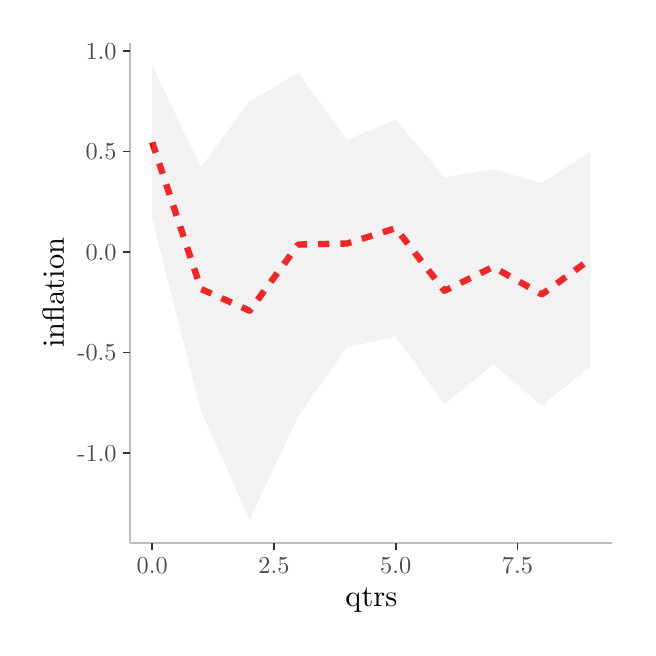
\begin{tikzpicture}[x=1pt,y=1pt]
\definecolor{fillColor}{RGB}{255,255,255}
\path[use as bounding box,fill=fillColor,fill opacity=0.00] (0,0) rectangle (216.81,216.81);
\begin{scope}
\path[clip] (  0.00,  0.00) rectangle (216.81,216.81);
\definecolor{drawColor}{RGB}{255,255,255}
\definecolor{fillColor}{RGB}{255,255,255}

\path[draw=drawColor,line width= 0.6pt,line join=round,line cap=round,fill=fillColor] (  0.00,  0.00) rectangle (216.81,216.81);
\end{scope}
\begin{scope}
\path[clip] ( 37.09, 30.69) rectangle (211.31,211.31);
\definecolor{drawColor}{RGB}{255,255,255}

\path[draw=drawColor,line width= 0.6pt,line join=round] ( 37.09, 63.13) --
	(211.31, 63.13);

\path[draw=drawColor,line width= 0.6pt,line join=round] ( 37.09, 99.43) --
	(211.31, 99.43);

\path[draw=drawColor,line width= 0.6pt,line join=round] ( 37.09,135.73) --
	(211.31,135.73);

\path[draw=drawColor,line width= 0.6pt,line join=round] ( 37.09,172.03) --
	(211.31,172.03);

\path[draw=drawColor,line width= 0.6pt,line join=round] ( 37.09,208.33) --
	(211.31,208.33);

\path[draw=drawColor,line width= 0.6pt,line join=round] ( 45.01, 30.69) --
	( 45.01,211.31);

\path[draw=drawColor,line width= 0.6pt,line join=round] ( 89.00, 30.69) --
	( 89.00,211.31);

\path[draw=drawColor,line width= 0.6pt,line join=round] (133.00, 30.69) --
	(133.00,211.31);

\path[draw=drawColor,line width= 0.6pt,line join=round] (176.99, 30.69) --
	(176.99,211.31);
\definecolor{drawColor}{RGB}{255,0,0}

\path[draw=drawColor,line width= 2.3pt,dash pattern=on 4pt off 4pt ,line join=round] ( 45.01,175.40) --
	( 62.61,122.40) --
	( 80.20,114.53) --
	( 97.80,138.45) --
	(115.40,138.82) --
	(133.00,144.35) --
	(150.60,121.73) --
	(168.19,130.35) --
	(185.79,120.44) --
	(203.39,133.18);
\definecolor{fillColor}{RGB}{190,190,190}

\path[fill=fillColor,fill opacity=0.20] ( 45.01,203.10) --
	( 62.61,166.37) --
	( 80.20,190.17) --
	( 97.80,200.42) --
	(115.40,176.24) --
	(133.00,183.55) --
	(150.60,162.74) --
	(168.19,165.60) --
	(185.79,160.67) --
	(203.39,171.96) --
	(203.39, 94.40) --
	(185.79, 80.20) --
	(168.19, 95.09) --
	(150.60, 80.72) --
	(133.00,105.16) --
	(115.40,101.40) --
	( 97.80, 76.48) --
	( 80.20, 38.90) --
	( 62.61, 78.43) --
	( 45.01,147.69) --
	cycle;

\path[] ( 45.01,203.10) --
	( 62.61,166.37) --
	( 80.20,190.17) --
	( 97.80,200.42) --
	(115.40,176.24) --
	(133.00,183.55) --
	(150.60,162.74) --
	(168.19,165.60) --
	(185.79,160.67) --
	(203.39,171.96);

\path[] (203.39, 94.40) --
	(185.79, 80.20) --
	(168.19, 95.09) --
	(150.60, 80.72) --
	(133.00,105.16) --
	(115.40,101.40) --
	( 97.80, 76.48) --
	( 80.20, 38.90) --
	( 62.61, 78.43) --
	( 45.01,147.69);
\end{scope}
\begin{scope}
\path[clip] (  0.00,  0.00) rectangle (216.81,216.81);
\definecolor{drawColor}{RGB}{190,190,190}

\path[draw=drawColor,line width= 0.6pt,line join=round] ( 37.09, 30.69) --
	( 37.09,211.31);
\end{scope}
\begin{scope}
\path[clip] (  0.00,  0.00) rectangle (216.81,216.81);
\definecolor{drawColor}{gray}{0.30}

\node[text=drawColor,anchor=base east,inner sep=0pt, outer sep=0pt, scale=  0.88] at ( 32.14, 60.10) {-1.0};

\node[text=drawColor,anchor=base east,inner sep=0pt, outer sep=0pt, scale=  0.88] at ( 32.14, 96.40) {-0.5};

\node[text=drawColor,anchor=base east,inner sep=0pt, outer sep=0pt, scale=  0.88] at ( 32.14,132.70) {0.0};

\node[text=drawColor,anchor=base east,inner sep=0pt, outer sep=0pt, scale=  0.88] at ( 32.14,169.00) {0.5};

\node[text=drawColor,anchor=base east,inner sep=0pt, outer sep=0pt, scale=  0.88] at ( 32.14,205.30) {1.0};
\end{scope}
\begin{scope}
\path[clip] (  0.00,  0.00) rectangle (216.81,216.81);
\definecolor{drawColor}{gray}{0.20}

\path[draw=drawColor,line width= 0.6pt,line join=round] ( 34.34, 63.13) --
	( 37.09, 63.13);

\path[draw=drawColor,line width= 0.6pt,line join=round] ( 34.34, 99.43) --
	( 37.09, 99.43);

\path[draw=drawColor,line width= 0.6pt,line join=round] ( 34.34,135.73) --
	( 37.09,135.73);

\path[draw=drawColor,line width= 0.6pt,line join=round] ( 34.34,172.03) --
	( 37.09,172.03);

\path[draw=drawColor,line width= 0.6pt,line join=round] ( 34.34,208.33) --
	( 37.09,208.33);
\end{scope}
\begin{scope}
\path[clip] (  0.00,  0.00) rectangle (216.81,216.81);
\definecolor{drawColor}{RGB}{190,190,190}

\path[draw=drawColor,line width= 0.6pt,line join=round] ( 37.09, 30.69) --
	(211.31, 30.69);
\end{scope}
\begin{scope}
\path[clip] (  0.00,  0.00) rectangle (216.81,216.81);
\definecolor{drawColor}{gray}{0.20}

\path[draw=drawColor,line width= 0.6pt,line join=round] ( 45.01, 27.94) --
	( 45.01, 30.69);

\path[draw=drawColor,line width= 0.6pt,line join=round] ( 89.00, 27.94) --
	( 89.00, 30.69);

\path[draw=drawColor,line width= 0.6pt,line join=round] (133.00, 27.94) --
	(133.00, 30.69);

\path[draw=drawColor,line width= 0.6pt,line join=round] (176.99, 27.94) --
	(176.99, 30.69);
\end{scope}
\begin{scope}
\path[clip] (  0.00,  0.00) rectangle (216.81,216.81);
\definecolor{drawColor}{gray}{0.30}

\node[text=drawColor,anchor=base,inner sep=0pt, outer sep=0pt, scale=  0.88] at ( 45.01, 19.68) {0.0};

\node[text=drawColor,anchor=base,inner sep=0pt, outer sep=0pt, scale=  0.88] at ( 89.00, 19.68) {2.5};

\node[text=drawColor,anchor=base,inner sep=0pt, outer sep=0pt, scale=  0.88] at (133.00, 19.68) {5.0};

\node[text=drawColor,anchor=base,inner sep=0pt, outer sep=0pt, scale=  0.88] at (176.99, 19.68) {7.5};
\end{scope}
\begin{scope}
\path[clip] (  0.00,  0.00) rectangle (216.81,216.81);
\definecolor{drawColor}{RGB}{0,0,0}

\node[text=drawColor,anchor=base,inner sep=0pt, outer sep=0pt, scale=  1.10] at (124.20,  7.64) {qtrs};
\end{scope}
\begin{scope}
\path[clip] (  0.00,  0.00) rectangle (216.81,216.81);
\definecolor{drawColor}{RGB}{0,0,0}

\node[text=drawColor,rotate= 90.00,anchor=base,inner sep=0pt, outer sep=0pt, scale=  1.10] at ( 13.08,121.00) {inflation};
\end{scope}
\end{tikzpicture}
